% This file is part of GUFI, which is part of MarFS, which is released
% under the BSD license.
%
%
% Copyright (c) 2017, Los Alamos National Security (LANS), LLC
% All rights reserved.
%
% Redistribution and use in source and binary forms, with or without modification,
% are permitted provided that the following conditions are met:
%
% 1. Redistributions of source code must retain the above copyright notice, this
% list of conditions and the following disclaimer.
%
% 2. Redistributions in binary form must reproduce the above copyright notice,
% this list of conditions and the following disclaimer in the documentation and/or
% other materials provided with the distribution.
%
% 3. Neither the name of the copyright holder nor the names of its contributors
% may be used to endorse or promote products derived from this software without
% specific prior written permission.
%
% THIS SOFTWARE IS PROVIDED BY THE COPYRIGHT HOLDERS AND CONTRIBUTORS "AS IS" AND
% ANY EXPRESS OR IMPLIED WARRANTIES, INCLUDING, BUT NOT LIMITED TO, THE IMPLIED
% WARRANTIES OF MERCHANTABILITY AND FITNESS FOR A PARTICULAR PURPOSE ARE DISCLAIMED.
% IN NO EVENT SHALL THE COPYRIGHT HOLDER OR CONTRIBUTORS BE LIABLE FOR ANY DIRECT,
% INDIRECT, INCIDENTAL, SPECIAL, EXEMPLARY, OR CONSEQUENTIAL DAMAGES (INCLUDING,
% BUT NOT LIMITED TO, PROCUREMENT OF SUBSTITUTE GOODS OR SERVICES; LOSS OF USE,
% DATA, OR PROFITS; OR BUSINESS INTERRUPTION) HOWEVER CAUSED AND ON ANY THEORY OF
% LIABILITY, WHETHER IN CONTRACT, STRICT LIABILITY, OR TORT (INCLUDING NEGLIGENCE
% OR OTHERWISE) ARISING IN ANY WAY OUT OF THE USE OF THIS SOFTWARE, EVEN IF
% ADVISED OF THE POSSIBILITY OF SUCH DAMAGE.
%
%
% From Los Alamos National Security, LLC:
% LA-CC-15-039
%
% Copyright (c) 2017, Los Alamos National Security, LLC All rights reserved.
% Copyright 2017. Los Alamos National Security, LLC. This software was produced
% under U.S. Government contract DE-AC52-06NA25396 for Los Alamos National
% Laboratory (LANL), which is operated by Los Alamos National Security, LLC for
% the U.S. Department of Energy. The U.S. Government has rights to use,
% reproduce, and distribute this software.  NEITHER THE GOVERNMENT NOR LOS
% ALAMOS NATIONAL SECURITY, LLC MAKES ANY WARRANTY, EXPRESS OR IMPLIED, OR
% ASSUMES ANY LIABILITY FOR THE USE OF THIS SOFTWARE.  If software is
% modified to produce derivative works, such modified software should be
% clearly marked, so as not to confuse it with the version available from
% LANL.
%
% THIS SOFTWARE IS PROVIDED BY LOS ALAMOS NATIONAL SECURITY, LLC AND CONTRIBUTORS
% "AS IS" AND ANY EXPRESS OR IMPLIED WARRANTIES, INCLUDING, BUT NOT LIMITED TO,
% THE IMPLIED WARRANTIES OF MERCHANTABILITY AND FITNESS FOR A PARTICULAR PURPOSE
% ARE DISCLAIMED. IN NO EVENT SHALL LOS ALAMOS NATIONAL SECURITY, LLC OR
% CONTRIBUTORS BE LIABLE FOR ANY DIRECT, INDIRECT, INCIDENTAL, SPECIAL,
% EXEMPLARY, OR CONSEQUENTIAL DAMAGES (INCLUDING, BUT NOT LIMITED TO, PROCUREMENT
% OF SUBSTITUTE GOODS OR SERVICES; LOSS OF USE, DATA, OR PROFITS; OR BUSINESS
% INTERRUPTION) HOWEVER CAUSED AND ON ANY THEORY OF LIABILITY, WHETHER IN
% CONTRACT, STRICT LIABILITY, OR TORT (INCLUDING NEGLIGENCE OR OTHERWISE) ARISING
% IN ANY WAY OUT OF THE USE OF THIS SOFTWARE, EVEN IF ADVISED OF THE POSSIBILITY
% OF SUCH DAMAGE.



\section{Rollup}
One major optimization implemented in GUFI is rollups. Rolling up can
be viewed as flattening the contents of the index while taking into
consideration the permissions of each directory. Rolling up results in
the overall number of directories that need to be processed being
reduced (usually) significantly while still obtaining the same results
as an unmodifed index.

\subsection{Bottlenecks}
During querying, every single directory runs a fixed set of
operations:

\begin{itemize}
  \item \texttt{opendir(3)}
  \item \texttt{readdir(3)} (Looped)
  \item \texttt{sqlite3\_open\_v2}
  \item \texttt{sqlite3\_exec\_v2}
  \item \texttt{sqlite3\_close(3)}
  \item \texttt{closedir(3)}
\end{itemize}

Each of these operations have costs associated with them. Some are
fixed and some depend on the shape and contents of the index. Reducing
the number of directories processed allows for fixed costs to be
amortized.

\subsection{Rules}
\label{rolluprules}
\subsubsection{Whether or not a directory {\it CAN} roll up}
In order for a child directory to be allowed to roll up into its
parent directory, it must follow two rules. First, all of its children
must be rolled up. Second, all of its children must have permissions
that satisfy any one of the following conditions with the parent.

\begin{itemize}
  \item World readable and executable (o+rx)
  \item Matching user, group, and others permissions, with the same
    user and group
  \item Matching user and group permissions, readable and executable
    (ug+rx) with the same user and group, and not world readable and
    excutable (o-rx)
  \item Matching user permissions, readable and executable (u+rx) with
    the same user and not group or world readable and executable
    (go-rx)
\end{itemize}

Note that because leaf directories have no children with which to have
conflicting permission with, they are considered rolled up.

\subsubsection{Whether or not a directory {\it SHOULD} roll up}
In addition to the permission-based rules that determine whether or
not a directory can roll up, we also have a small check to say whether
or not a directory should roll up.

As data is rolled upwards in the index, databases towards the top will
accumulate more and more data from its subtrees. If directories are
allowed to roll up without limit, some databases will become
significantly larger than others, causing large amounts of tail
latency.

The \rollup executable has the \texttt{-L} flag that limits the number
of entries that may be found within a single directory.

\subsection{Steps}
The processing of rolling up involves a number of steps that update
the tables of the parent directory.

First, the target directory is checked to ensure it can roll its
children into itself using the rules listed in
\ref{rolluprules}. Once it has been determined that the diretory
being processed can and should roll up, the tables of each child are
copied into the parent:

\begin{enumerate}
\item The contents of the child's summary table are copied up with the
  name column updated to include the parent directory and the
  \texttt{isroot} column set to 0 in the parent
\item The \pentries view is dropped
\item The \pentries table is created
\item The original contents of the \pentries view is recreated in the
  \pentries table
\item The child's \pentries table/view is copied into parent
\end{enumerate}

\begin{figure} [ht]
  \centering
  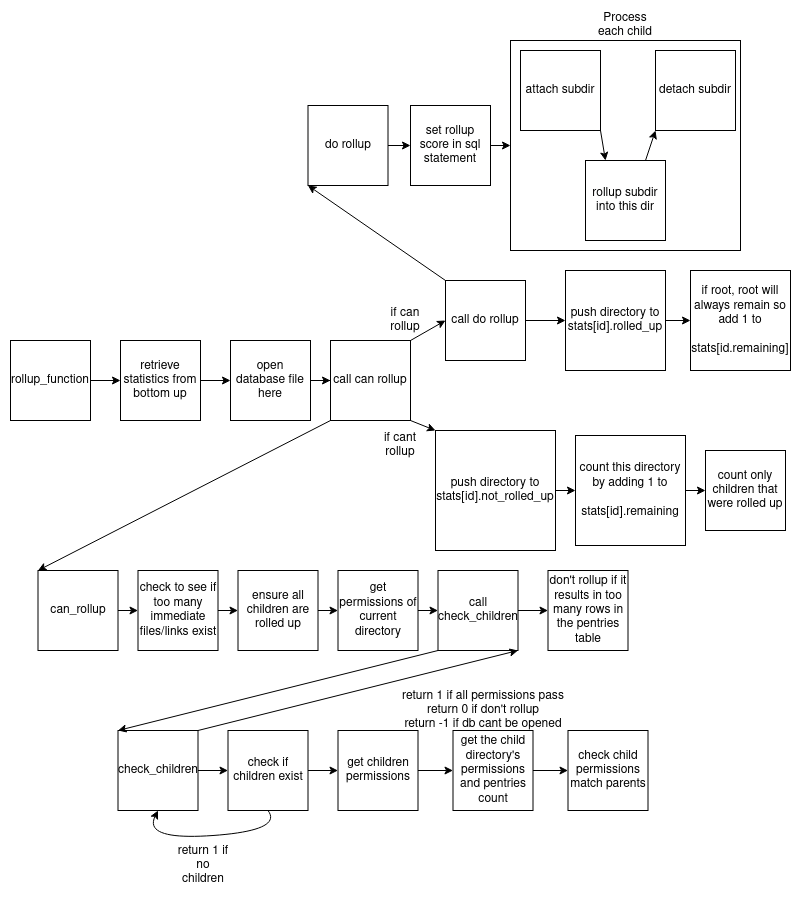
\includegraphics[width=\textwidth]{images/rollup_function.png}
  \caption{Rollup Function Diagram}
\end{figure}

\subsection{\texttt{rollup} executable}
Below is a diagram showing the overall structure of the \rollup
executable. The \rollup executable uses the BottomUp library (see
sec:BottumUp) to recursively descend the original index and only
perform the rollup operation once all children have been processed.

\begin{sidewaysfigure} [ht]
  \centering 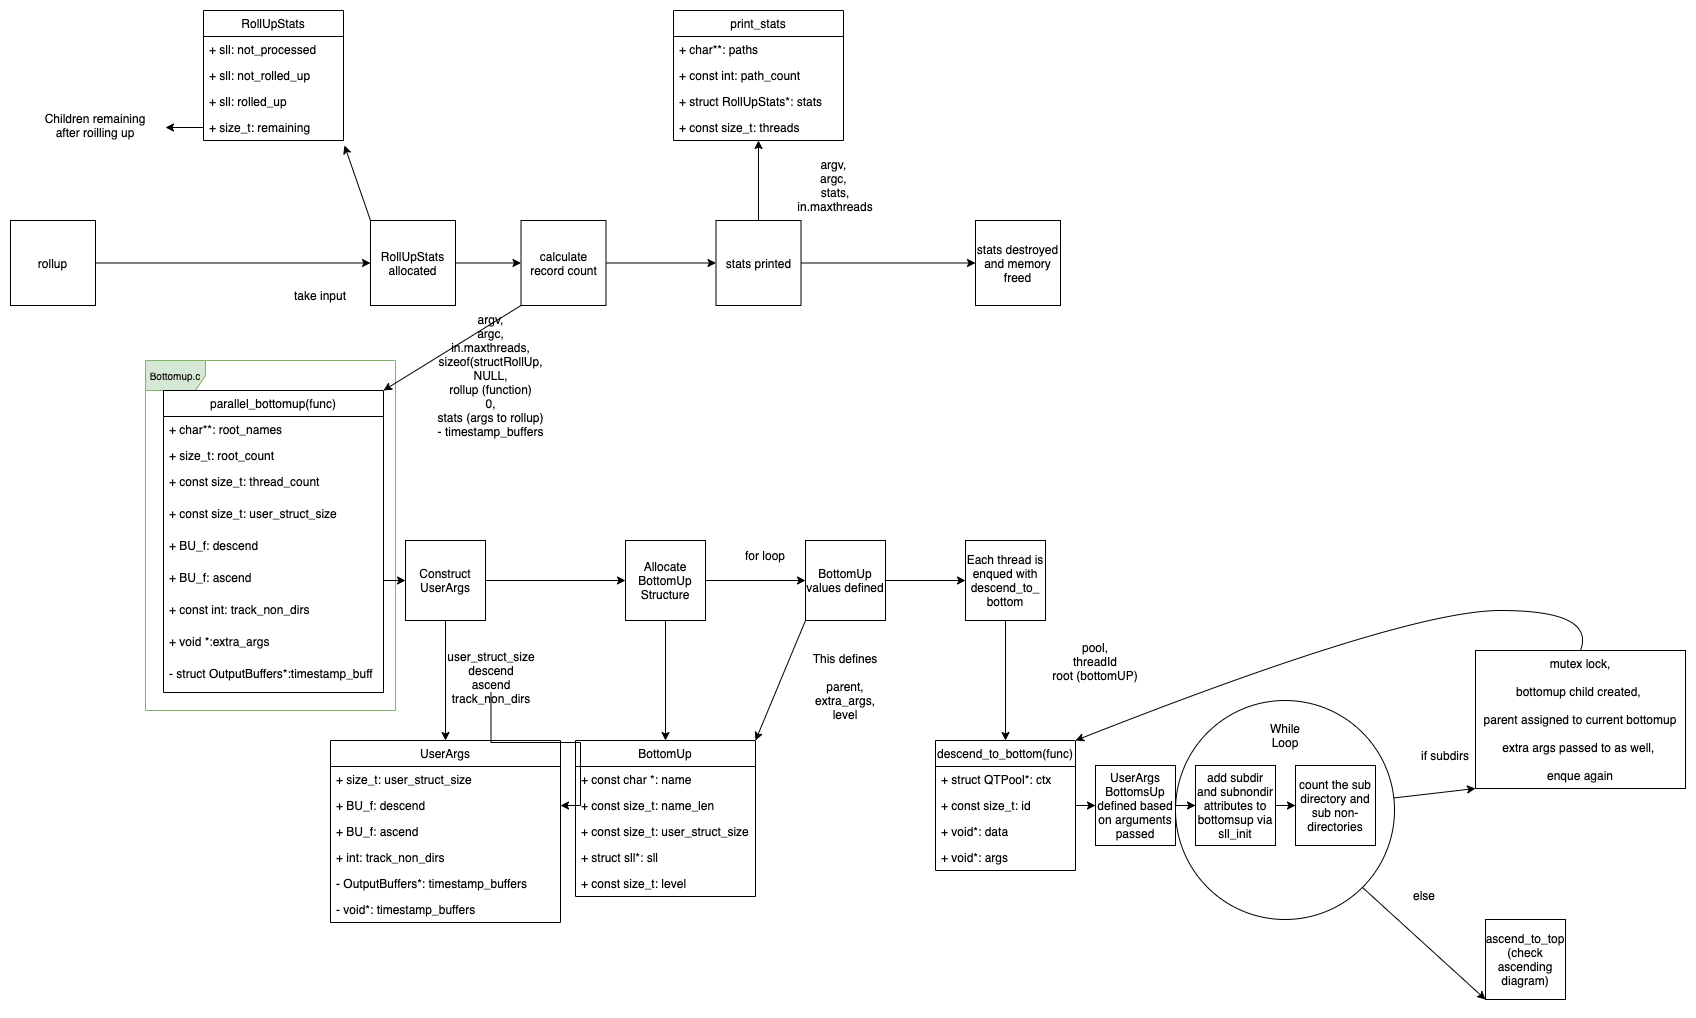
\includegraphics[width=\textwidth]{images/rollup.png}
  \caption{\rollup Workflow}
\end{sidewaysfigure}
